\documentclass[twosided]{report}

% Packages %
\usepackage{fancyhdr}
\usepackage{titling}
\usepackage{amsmath}
\usepackage{graphicx}
\usepackage{amssymb}
\usepackage{amsthm}
\usepackage{array}
\usepackage{pifont}
\usepackage{color}
\usepackage{listings}
\usepackage{algorithm}
\usepackage{algorithmic}

% Stylings %
\pagestyle{fancy}

% Commands %
\newcommand{\subtitle}[1]{%
  \posttitle{%
    \par\end{center}
    \begin{center}\large#1\end{center}
    \vskip0.5em}%
}

% Footer/Header %
\fancyhead[LE,RO]{\slshape Chapter \thechapter}
\fancyhead[LO,RE]{\slshape \rightmark}
\fancyfoot[C]{\thepage}

\begin{document}

\lstdefinelanguage{pseudo}{
	morekeywords={if, else, for, in, remove, from, case, do, forever, to, False, True},
	sensitive=true,
	morecomment=[l]\#,
	morestring=[b]',
	frame=single,
	caption={Algorithm}
}

\title{OpenNemID 
	\\Bachelor project - Spring 2013}
\subtitle{Verified Secure Open Source Alternative to NemID}
\author{
  Andreas Hallberg Kjeldsen\\
  \texttt{ahal@itu.dk}
  \and
  Morten Chabert Eskesen\\
  \texttt{mche@itu.dk}
}

\date{May 22, 2013}
\maketitle

\begin{abstract}
Your abstract goes here...
\end{abstract}

\tableofcontents 

\chapter{Introduction}

$\ldots$
\par
We're extending the work done by Jacob Højgaard in his Masters Thesis 'Securing Single Sign-On Systems With Executable Models'. Jacobs research has focused on the current implementation of NemID and therefore describes, outlines and models the current system used in Denmark as of May 2013.

\section{Objectives}
Some explaining text here
\par

\begin{enumerate}
	\item Describe and outline the OpenNemID protocol, including but not limited to registration and login.
	\item Formalize the specification of OpenNemID in F* to the extent possible.
\end{enumerate}

\section{Scope}
This project has had it focus towards specifying a new protocol that could replace NemID. The intent of this project is therefore not to develop a complete system, but to make the specification for a system that could then later be developed based on the specification.

\section{Background}
$\ldots$
 
\chapter{Static analysis}
Smart stuff here


%%%%%%%%%% CHAPTER %%%%%%%%%%
\chapter{Remodelling the protocol}

\section{Communication Model}
The communication model displays a graphical overview of how data should be communicated between the involved parties.
\newpage
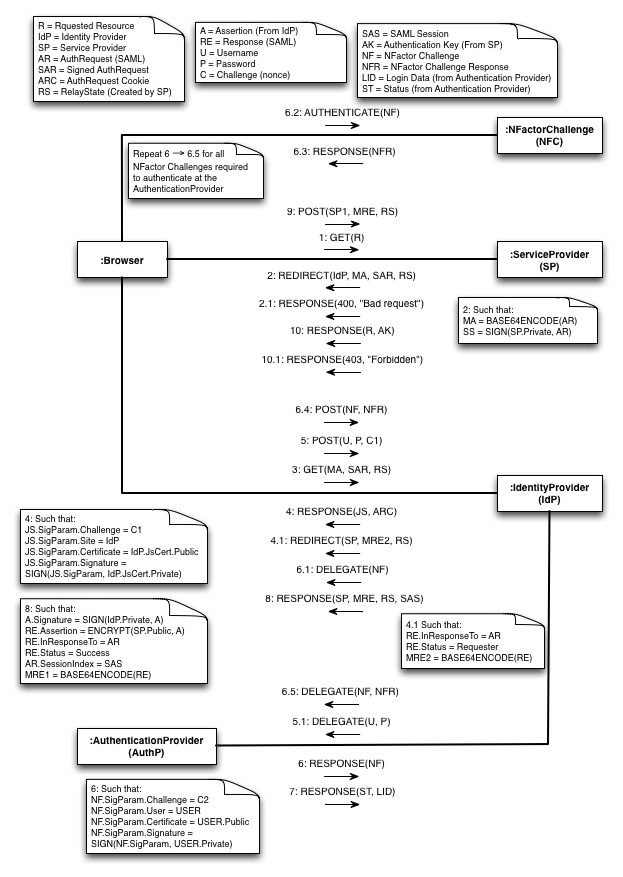
\includegraphics[scale=0.6]{images/Communication.png}

TEXT DESCRIBING ALGORITHM 1
\begin{algorithm}[H]
	\caption{Process 1}
	\begin{algorithmic}
	\REQUIRE{GET is well-formed \AND IdP.Public \AND SP.Private}
	\IF{R exists}
		\STATE AR $\leftarrow$ CreateAuthnRequest()
		\STATE SS $\leftarrow$ SIGN(M, SP.Private)
		\STATE MA $\leftarrow$ UrlEnc(Base64Enc(DeflateCompress(AR)))
		\STATE RS $\leftarrow$ UrlEnc(Base64Enc(R))
		\RETURN REDIRECT(IdP, MA, SS, RS)
	\ELSE
		\RETURN RESPONSE(400, Bad−Request)
	\ENDIF
	\end{algorithmic}
\end{algorithm}

TEXT DESCRIBING ALGORITHM 2
\begin{algorithm}[H]
	\caption{Process 3}
	\begin{algorithmic}
		\REQUIRE{GET is well-formed \AND IdP.Private \AND SP.Public \AND IdPJsCert.Public \AND IdP has JavaScript from AuthP}
		\STATE AR $\leftarrow$ DeflateDecompress(Base64Dec(UrlDec(MA)))
		\IF{VERIFY(AR, SS, SP.Public)}
			\STATE C $\leftarrow$ GenChallenge()
			\STATE JS $\leftarrow$ StoredJavaScript()
			\STATE JS.SigParams.Challenge $\leftarrow$ C
			\STATE JS.SigParams.Certificate $\leftarrow$ IdPJsCert.Public
			\STATE JS.SigParams.Signature $\leftarrow$ SIGN(JS.SigParams, IdPJsCert.Private)
			\RETURN RESPONSE(JS)
		\ELSE
			\STATE RE $\leftarrow$ CreateResponse()
			\STATE RE.InResponseTo $\leftarrow$ AR.Id
			\STATE RE.Status $\leftarrow$ ”Requester”
			\STATE MRE $\leftarrow$ Base64Enc(RE)
			\RETURN REDIRECT(SP, MRE, RS)
		\ENDIF
	\end{algorithmic}
\end{algorithm}

TEXT DESCRIBING ALGORITHM 3
\begin{algorithm}[H]
	\caption{Process 4}
	\begin{algorithmic}
		\REQUIRE{U \AND P \AND Browser allows JavaScript}
		\STATE SigParams $\leftarrow$ Js.SigParams
		\IF{VERIFY(SigParams, SigParams.Signature, SigParams.Certificate)}
			\STATE C1 $\leftarrow$ SigParams.Challenge
			\RETURN POST(U, P, C1)
		\ELSE
			\PRINT ERROR
		\ENDIF
	\end{algorithmic}
\end{algorithm}

TEXT DESCRIBING ALGORITHM 4
\begin{algorithm}[H]
	\caption{Process 5}
	\begin{algorithmic}
		\REQUIRE{POST is well formed}
		\IF{C1 matches challenge issued by IdP}
			\STATE \textbf{Delegate} U \AND P \TO AuthP
		\ELSE
			\RETURN RESPONSE(ERROR)
		\ENDIF
		\REQUIRE{C1 matches challenge issued by IdP}
	\end{algorithmic}
\end{algorithm}

TEXT DESCRIBING ALGORITHM 5
\begin{algorithm}[H]
	\caption{Process 5.1}
	\begin{algorithmic}
		\STATE USER $\leftarrow$ GetUser(U, P)
		\IF{USER is valid}
			\STATE C2 $\leftarrow$ GenChallenge()
			\STATE NF $\leftarrow$ GetNextNFactorChallenge(USER)
			\STATE NF.SigParam.User = USER.id
			\STATE NF.SigParam.Challenge $\leftarrow$ C2
			\STATE NF.SigParam.Certificate $\leftarrow$ USER.Public
			\STATE NF.SigParam.Signature $\leftarrow$ SIGN(NF.SigParam, USER.Private)
			\RETURN RESPONSE(NF)
		\ELSE
			\RETURN RESPONSE(ERROR)
		\ENDIF
	\end{algorithmic}
\end{algorithm}

TEXT DESCRIBING ALGORITHM 6
\begin{algorithm}[H]
	\caption{Process 6}
	\begin{algorithmic}
		\STATE SigParams $\leftarrow$ NF.SigParams
		\IF{VERIFY(SigParams, SigParams.Signature, SigParams.Certificate)}
			\STATE RELATE(SigParams.User, SigParams.Challenge)
			\STATE \textbf{Delegate} NF \TO Browser
		\ELSE
			\STATE \textbf{Delegate} ERROR \TO Browser
		\ENDIF
	\end{algorithmic}
\end{algorithm}

TEXT DESCRIBING ALGORITHM 7
\begin{algorithm}[H]
	\caption{Process 6.1}
	\begin{algorithmic}
		\STATE SigParams $\leftarrow$ NF.SigParams
		\IF{VERIFY(SigParams, SigParams.Signature, SigParams.Certificate)}
			\STATE AUTHENTICATE(NF)
		\ELSE
			\PRINT ERROR
		\ENDIF
	\end{algorithmic}
\end{algorithm}

TEXT DESCRIBING ALGORITHM 8
\begin{algorithm}[H]
	\caption{Process 6.2}
	\begin{algorithmic}
		\STATE NFR $\leftarrow$ NFactorResult(NF)
		\RETURN RESPONSE(NFR)
	\end{algorithmic}
\end{algorithm}

TEXT DESCRIBING ALGORITHM 9
\begin{algorithm}[H]
	\caption{Process 6.5}
	\begin{algorithmic}
		\STATE SigParams $\leftarrow$ NF.SigParams
		\IF{VERIFY(SigParams, SigParams.Signature, SigParams.Certificate)}
			\IF{NFR is acceptable result of NF}
				\STATE USER $\leftarrow$ GetUser(SigParam.USER, SigParam.Certificate)
				\STATE C2 $\leftarrow$ GenChallenge()
				\IF{USER.HasNextChallenge}
					\STATE NF $\leftarrow$ GetNextNFactorChallenge(USER)
					\STATE NF.SigParam.User = USER.id
					\STATE NF.SigParam.Challenge $\leftarrow$ C2
					\STATE NF.SigParam.Certificate $\leftarrow$ USER.Public
					\STATE NF.SigParam.Signature $\leftarrow$ SIGN(NF.SigParam, USER.Private)
					\RETURN RESPONSE(NF)
				\ELSE
					\STATE LID $\leftarrow$ CreateLogInData()
					\STATE LID.SigParam.Challenge $\leftarrow$ C2
					\STATE LID.Certificate $\leftarrow$ USER.Public
					\STATE LID.Signature $\leftarrow$ SIGN(LID, USER.Private)
					\STATE ST $\leftarrow$ ”OK”
					\RETURN RESPONSE(ST, LID)
				\ENDIF
			\ELSE
				\RETURN RESPONSE(ERROR)
			\ENDIF
		\ELSE
			\RETURN RESPONSE(ERROR)
		\ENDIF	
	\end{algorithmic}
\end{algorithm}

TEXT DESCRIBING ALGORITHM 10
\begin{algorithm}[H]
	\caption{Process 7}
	\begin{algorithmic}
		\IF{VERIFY(LID, LID.Signature, LID.Certificate)}
			\IF{ST = "OK"}
				\STATE MA $\leftarrow$ ARC.AR
				\STATE SS $\leftarrow$ ARC.SS
				\STATE RS $\leftarrow$ ARC.RS
				\STATE AR $\leftarrow$ DeflateDecompress(Base64Dec(UrlDec(MA)))
				\IF{VERIFY(AR, SS, SP.Public)}
					\STATE A $\leftarrow$ BuildAssertion(LID.Certificate)
					\STATE SI $\leftarrow$ GenerateSessionIndex()
					\STATE A.InResponseTo $\leftarrow$ AR.Id
					\STATE A.Issuer $\leftarrow$ IdpP.Id
					\STATE A.Audience $\leftarrow$ SP.Id
					\STATE A.SessionIndex $\leftarrow$ SI
					\STATE A.Signature $\leftarrow$ SIGN(A, IdP.Private)
					\STATE EA $\leftarrow$ ENCRYPT(A, SP.Public)
					\STATE RE $\leftarrow$ CreateResponse()
					\STATE RE.Assertion $\leftarrow$ EA
					\STATE RE.InResponseTo $\leftarrow$ AR.Id
					\STATE Re.Status $\leftarrow$ "Success"
					\STATE MRE $\leftarrow$ Base64Enc(RE)
					\STATE SAS $\leftarrow$ CreateSAMLSession(SI, SP.Id, LID.CertificateSubject)
					\RETURN REDIRECT(SP, MRE, RS, SAS)
				\ELSE
					\STATE RE $\leftarrow$ CreateResponse()
					\STATE RE.InResponseTo $\leftarrow$ AR.Id
					\STATE RE.Status $\leftarrow$ "Requester"
					\STATE MRE $\leftarrow$ Base64Enc(RE)
					\RETURN REDIRECT(SP, MRE, RS)
				\ENDIF	
			\ELSE
				\RETURN RESPONSE(ST)
			\ENDIF
		\ELSE
			\RETURN RESPONSE(ERROR)
		\ENDIF
	\end{algorithmic}
\end{algorithm}

TEXT DESCRIBING ALGORITHM 11
\begin{algorithm}[H]
	\caption{Process 9}
	\begin{algorithmic}
		\REQUIRE{POST is well.formed \AND SP.Private \AND IdP.Public}
		\STATE RE $\leftarrow$ Base64Dec(MRE)
		\STATE A $\leftarrow$ DECRYPT(RE.Assertion, SP.Private)
		\IF{VERIFY(A, A.Signature, IdP.Public)}
			\STATE AK $\leftarrow$ GenAuthKey()
			\STATE R $\leftarrow$ Base64Dec(UrlDec(RS))
			\STATE RES $\leftarrow$ GetResource(R)
			\RETURN RESPONSE(RES, AK)
		\ELSE
			\RETURN RESPONSE(403, Forbidden)
		\ENDIF
	\end{algorithmic}
\end{algorithm}

\end{document}